\documentclass{standalone}
\usepackage{tikz,ctex}
\usepackage{tikz-3dplot} % 2-1
\usepackage{unicode-math} % 2-5,4-1,4-2
\setmathfont{Fira Math Regular}
\setmainfont{Fira Sans}
\definecolor{background}{RGB}{239, 239, 239} % 4-5,6-2,6-5
\begin{document}
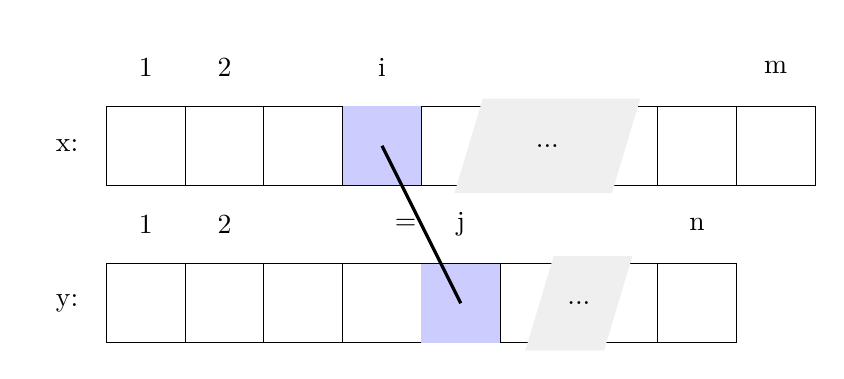
\begin{tikzpicture}[every node/.style={rectangle,minimum size=1cm}]
\foreach \x/\y/\text in {-1/2/x:,-1/0/y:,3/3/i,4/1/j,3.3/1/=,8/3/m,7/1/n}{
    \node at(\x,\y){\text};}
\foreach \x in {1,2}
    \foreach \y in {0,2}{
        \node at (-1+\x,1+\y) {\x};} 
\foreach \x in {0,...,8}{
    \node[draw] at (\x,2){};}
\foreach \x in {0,...,7}{
    \node[draw] at (\x,0){};}
\node[fill=blue!20] at (4,0){} ; 
\node[fill=blue!20] at (3,2){} ; 
\draw[very thick] (3,2) --(4,0) ;
\fill[xslant=.3,background] (3.5,1.4) rectangle (5.5,2.6) node[midway,black]{...};
\fill[xslant=.3,background] (5,-.6) rectangle (6,.6) node[midway,black]{...};
\end{tikzpicture}
\end{document}